\begin{definition}
    \[\nabla\colon \Gamma(TM)\times \Gamma (TM)\to \Gamma(TM)\]
    \[(X,Y)\mapsto \nabla_X Y\]
    is called the affine connection on \(M\).
\end{definition}
\underline{Fact}: There are many such affine connections!

In practice, we need local expressions of \(\nabla_V W\). Let 
\((x^1,\ldots,x^n)\) be a local coordinate on \(U\subset M\), 
\(V=V^i\pdv{x^i},W=W^i\pdv{x^i}\), then
\begin{align*}
    \nabla_V W &=\nabla_{V^i\pdv{x^i}}\left(W^j\pdv{x^j}\right)\\
    &= V^i\nabla_{\pdv{x^i}}\left(W^j \pdv{x^j}\right)\\
    &=V^i\left(\left(\nabla_{\pdv{x^i}} W^j\right)\pdv{x^j}
    + W^j \nabla_{\pdv{x^i}} \pdv{x^j}\right)\\
    &=V^i\left(\pdv{W^j}{x^i}\pdv{x^j}+W^j
    \boxed{\nabla_{\pdv{x^i}}\pdv{x^j}}\right).
\end{align*}
\begin{definition}
    On \(U\), we define the Christoffel symbol by 
    \[
        \nabla_{\pdv{x^i}}\pdv{x^j}=\Gamma\indices*{_{ij}^k}\pdv{x^k}.
    \]
    (Here, one should compare this definition with the Christoffel
    symbol introduced in the study of equation of motion 
    in previous lectures).
\end{definition}
\[
    \Rightarrow \nabla_V W= V^i\left(\pdv{W^j}{x^i}+W^k\Gamma
    \indices*{_{ki}^j}\right)\pdv{x^j}   .
\]
Conventionally, we define
\[
    \nabla_i W^j=\pdv{W^j}{x^i}+\Gamma\indices*{_{ik}^j}W^k    
\]
\begin{itemize}
    \item \(\nabla_i W^j\): Taking covariant derivative 
    of \(j\)-th component of \(W\) along the \(i\)-th coordinate
    direction.
    \item \(\pdv{W^j}{x^i}\): Euclidean derivative.
    \item \(\Gamma\indices*{_{ik}^j}W^k\): Correction term.
\end{itemize}
This notion is frequently used in geometry references.

Again, because there are tons of selection of affine connections,
this yields many choices of \(\Gamma\indices*{_{ij}^k}\)!
After we introduce the Riemannian metric, we shall see there is a unique
affine connection compatible with the Riemannian metric.
\begin{definition}[Riemannian metric]
    Let \(M\) be a smooth manifold. A Riemannian metric on \(M\)
    is a smooth map 
    \[
     g\colon \Gamma(TM)\times \Gamma(TM)\to C^\infty(M),
    \]
    such that 
    \(\forall X,Y,Z\in \Gamma(TM), f\in C^\infty(M)\)
    there is the following 
    \begin{enumerate}[(1)]
        \item \(g(X,Y)=g(Y,X)\).(symmetry)
        \item \(g(X,X)\ge 0\), and equality achieves iff \(X=0\).
        (positive definite)
        \item \(g(f X+Y,Z)=f\cdot g(X,Z)+g(Y,Z)\).(\(C^\infty\) linearity) 
    \end{enumerate}
    \((M,g)\) is called a Riemannian manifold.
\end{definition}
\begin{remark}
    At each \(p\in M\), \(g\) defines an inner product \(g_p\)
    on \(T_p M\). If we choose a coordinate chart near \(p\)
    with local coordinate \((x^1,\ldots,x^n)\),
    the local expression of \(g\) is written as 
    \[
        g=g_{ij}dx^i dx^j    ,
    \]
    where \(g_{ij}=g\left(\pdv{x^i},\pdv{x^j}\right)\).
\end{remark}
\begin{example}
    The \engordnumber{1} fundamental form on \(M\) is a Riemannian metric.
\end{example}
Using the Riemannian metric \(g\), we can define 
the length, area, angle, et.c.
\begin{definition}
    \begin{enumerate}[(1)]
        \item \(X\in \Gamma(TM)\), \(|X|=\sqrt{g(X,X)}\).
        \item The volume density on \((M,g)\) is defined as 
        \[
            \dd V=\sqrt{\det(g_{ij})} dx^1\wedge\ldots \wedge dx^n .
        \]
        \item The volume of a bounded region \(B\) is 
        \[
            V(B)=\int_B 1 \dd V
        \]
    \end{enumerate}
\end{definition}
With the Riemannian metric introduced, we can uniquely determine
an affine connection compatible with the Riemannian metric.
\begin{theorem}
    Let \((M,g)\) be a Riemannian manifold, then there is a unique
    affine connection 
    \(\nabla\colon \Gamma(TM)\times \Gamma (TM)\to \Gamma(TM)\)
    satisfying following conditions: \(\forall X,Y,Z\)
    \begin{enumerate}[(1)]
        \item \(\nabla_Z \left(g(X,Y)\right)=g\left(
            \nabla_Z X,Y\right)+g(X,\nabla_Z Y)\).(Compatible with metric 
            \(g\))\footnotemark
        \item \(\nabla_X Y-\nabla_Y X=[X,Y]\).(Torsion free)
    \end{enumerate}
    \footnotetext{(1) is also equivalent to \(\nabla g=0\). 
    (We shall talk about this later)}
    The connection \(\nabla\) is called Levi-Civita connection.
\end{theorem}
Locally, take \(X=\pdv{x^i},Y=\pdv{x^j},Z=\pdv{x^k}\)
\begin{align*}
    (1)&\Rightarrow \pdv{g_{ij}}{x^k}=\Gamma\indices*{_{ki}^l}g_{lj}
    +\Gamma\indices*{_{kj}^l}g_{l i}    \\
    (2)&\Rightarrow \Gamma\indices*{_{ij}^k}=\Gamma\indices*{_{ji}^k}.
\end{align*}
\begin{exercise}
    Show that 
    \[
        \Gamma\indices*{_{ij}^k}=\frac{1}{2}g^{kl}\left(
            \pdv{g_{jl}}{x^i}+\pdv{g_{il}}{x^j}-\pdv{g_{ij}}{x^l}
        \right)    
    \]
    This is just the same expression as we see on.
    %打到这里的时候page142还不存在,到时候再做引用。
\end{exercise}
So far, we have defined \engordnumber{1} order derivatives (Lie derivative,
covariant derivative) on functions and vector fields. Next we shall consider
\engordnumber{2} order derivatives of a function and vector fields.
In particular, non-commutative nature of \engordnumber{2} order derivative
on vector fields will be captured by the ``curvature''.
    
Let's assume \(\nabla\) to be the Levi-Civita connection from now on.
\begin{itemize}
    \item Recall we have defined tangent bundle. 
    \(TM=\bigcup_{p\in M} T_p M\) is the collection of all 
    tangent vector spaces. As a vector space, \(T_p M\) is isomorphic 
    to \(\mathbb{R}^n\). Let \(T^*_p M=\)\{all covectors at \(p\)\}.
    We also let \(T^*M=\bigcup_{p\in M}T^*_p M=\bigcup_p 
    \left\{(p,\alpha)| \alpha\in T^*_p M\right\}\). Similar to the 
    \(TM\), one can endow a smooth structure on \(T^*M\) such that 
    it's a smooth manifold of dimension \(2\dim M\). We shall also 
    call an element of \(\Gamma(T^* M)\) a differential 1-form, 
    where \(\Gamma(T^*M)\) is the collection of all global covectors.
    \item We have introduced 
    \[
        \nabla \colon \Gamma(TM)\times C^\infty(M)\to C^\infty(M)
    \]
    \[
        (X,f)\mapsto \nabla_X f.    
    \]
    This map induces 
    \[
        \nabla f\colon \Gamma(TM)\to C^\infty(M).
    \]
    At each point \(p\in M\) this map is 
    \[
        X\mapsto \nabla_X f=\nabla f(X).    
    \]
    \(
        \nabla f(p)\colon T_p M\to \mathbb{R}\Rightarrow 
        \nabla f(p)\in T^*_p M\Rightarrow
        \nabla f\in \Gamma(T^* M)
    \).
\end{itemize}
\begin{remark}
    If \((x^1,\ldots, x^n)\) is local coordinate at \(p\). \(T_p M
    =\Span\{\pdv{x^1},\ldots,\pdv{x^n}\}\), then \(T^*_p M=\Span 
    \{d x^1,\ldots , d x^n\}\), \(dx^i\left(\pdv{x^j}\right)=\delta^i_j\)
    \[
        \Rightarrow \nabla f(p)=\pdv{f}{x^i} (p)dx^i=\nabla_i f\cdot 
        d x^i. \quad (\nabla_i f=\pdv{f}{x^i})    
    \]
\end{remark}
\begin{definition}
    The gradient vector field of \(f\), written as \(\mathrm{grad} f=
    \mathrm{grad}_g f \) is defined as \(\forall X\in \Gamma(TM)\)
    \[
        g(\mathrm{grad} f,X)=\nabla_X f=\nabla f(X).    
    \]
\end{definition}
Locally, 
\[
    \mathrm{grad} f=g^{ij}\pdv{f}{x^j}\pdv{x^i}=\nabla^i f\pdv{x^i}.
\]
\begin{definition}[Hessian of \(f\)]
    \[
        \nabla\nabla f\colon \Gamma(TM)\times \Gamma(TM)\to C^\infty(M)
    \]
    \[
        (X,Y)\mapsto \nabla\nabla f(X,Y).    
    \]
    Where \(\nabla\nabla f(X,Y)=\left(\nabla_X \nabla f\right)(Y)
    \footnotemark
    =\nabla_X
    \left(\nabla f(Y)\right)-\nabla f\left(\nabla_X Y\right)=
    X\left(Y f\right)-()\nabla_X Y) f\).
\end{definition}
\footnotetext{Note that here we haven't defined the covariant derivative of
 a 1-form}
 Locally: 
 \begin{align*}
    \nabla\nabla f\left(\pdv{x^i},\pdv{x^j}\right)&=
    \pdv{x^i}\left(\pdv{f}{x^j}\right)-\nabla_{\pdv{x^i}}\pdv{x^j} f\\
    &=\pdv{f}{x^i}{x^j}-\Gamma\indices*{_{ij}^k}\pdv{f}{x^k}.
 \end{align*}
 \begin{remark}
    \begin{enumerate}[(1)]
        \item We conventionally write \(\nabla\nabla f(\pdv{x^i}
        \pdv{x^j})=\nabla_i\nabla_j f\), \ie\ 
        \[
            \nabla_i\nabla_j f=
            \pdv{f}{x^i}{x^j}-\Gamma\indices*{_{ij}^k}\pdv{f}{x^k}.   
        \]
        \begin{itemize}
            \item \(\nabla_i\nabla_j f\): tensor component.
            \item \(\pdv{f}{x^i}{x^j}\): Euclidean Hessian.
            \item \(\Gamma\indices*{_{ij}^k}\pdv{f}{x^k}\)
            Correction.
        \end{itemize}
        \item \(\nabla_i\nabla_j f=\nabla_j\nabla_i f\).(Symmetric in 
        \(i\) and \(j\))
        \item In tensor notation we write this as 
        \[
            \nabla\nabla f=\left(\nabla_i\nabla_j f\right)d x^i d x^j.    
        \]
    \end{enumerate}
 \end{remark}
 \begin{definition}[Laplacian of \(f\)]
    \(\Delta f=\mathrm{trace}\left(\nabla\left(\mathrm{grad}
    f\right)\right)\).
 \end{definition}
 Locally, \(\mathrm{grad} f=\nabla^i f\pdv{x^i}\Rightarrow
 \nabla\left(\mathrm{grad}f\right)=\nabla_j\nabla^i f dx^j\otimes
  \pdv{x^i}\).
  \begin{align*}
    \Delta f & =\nabla_i \nabla^i f=g^{ij}\nabla_i\nabla_j f\\
    &=g^{ij}\left(
        \pdv{f}{x^i}{x^j}-\Gamma\indices*{_{ij}^k}\pdv{f}{x^k}
    \right).
  \end{align*}
  \begin{exercise}
    Show that 
    \[
        \Delta f=\frac{1}{\sqrt{\det g}}\pdv{x^i}\left(
            \sqrt{\det g}\cdot g^{ij}\pdv{f}{x^j}
        \right)    .
    \]
  \end{exercise}
  Note that the expression of R.H.S follows from
  ``integration by parts'', \ie\ \(\forall h\in C^\infty_c(M)\),
  \[
    \int_M  h\Delta f \sqrt{g}\dd x =-\int_M \left\langle
        \nabla h,\nabla f
    \right\rangle\sqrt{g}\dd x.
  \]
  Next, we consider taking \engordnumber{2} order derivative
  of a vector field \(Z\) along two different vector fields \(X\) and 
  \(Y\). Let's do a general local computation.(The following 
  computation should be very familiar with you)

  Let \(X=X^i\pdv{x^i},Y=Y^j\pdv{x^j},Z=Z^k\pdv{x^k}\)
  \begin{align*}
    \Rightarrow \nabla_X\nabla_Y Z&=
    \nabla_X\left(\nabla_Y Z\right)\\
    &=\nabla_X\left(\left(Y^j \nabla_j Z^k\right)\pdv{x^k}\right)\\
    &=\left(X^i\nabla_i Y^j\nabla_j Z^k+X^i Y^j\nabla_j\nabla_i Z^k
    \right)\pdv{x^k}\\
    \nabla_Y\nabla_X Z&=\left(Y^j\nabla_j X^i \nabla_i Z^k
    +X^iY^j \nabla_j\nabla_i Z^k\right)\pdv{x^k}
  \end{align*}
  \begin{align*}
    &\Rightarrow \nabla_X\nabla_Y Z-\nabla_Y\nabla_X Z\\
    &=
    X^i Y^j\left(\nabla_i\nabla_j Z^k-\nabla_j\nabla_i Z^k\right)
    \pdv{x^k}+\left(\nabla_{\nabla_X Y}Z^k-\nabla_{\nabla
    _Y X }Z^k\right)\pdv{x^k}\\
    &=X^i Y^j\left(\nabla_i\nabla_j Z^k-\nabla_j\nabla_i Z^k\right)
    \pdv{x^k}
    +\left(\nabla_{[X,Y]}Z^k\right)\pdv{x^k}.
  \end{align*}
  \(\therefore \nabla_X\nabla_Y Z-\nabla_Y\nabla_X Z -\nabla_{[X,Y]}Z=
  X^i Y^j\left(\nabla_i\nabla_j Z^k-\nabla_j\nabla_i Z^k\right)
    \pdv{x^k}
  \).
\begin{definition}
    The (1,3) Riemannian curvature tensor is defined by a map 
    \[
        R\colon \Gamma(TM)\times \Gamma(TM)\times \Gamma(TM)
        \to \Gamma(TM)    
    \]
    \[
        \left(X,Y,Z\right)\mapsto R(X,Y)Z    
    \]
    \[
        R(X,Y)Z=\nabla_X\nabla_Y Z-\nabla_Y\nabla_X Z -\nabla_{[X,Y]}Z    
    \]
    Locally, 
    \[
        R\left(\pdv{x^i},\pdv{x^j}\right)\pdv{x^k}=R\indices{_{ij}^l_k}
        \pdv{x^l}    
    \]
\end{definition}
\begin{exercise}
    \begin{enumerate}[(1)]
        \item Check \(R\) is \(C^\infty\) in \(X,Y,Z\).
        \item Find a local expression for \(R\indices{_{ij}^l_k}\)
        in terms of Christoffel symbols.
    \end{enumerate}
\end{exercise}
Computation: take \(X=\pdv{x^i}\), \(Y=\pdv{x^j}\), \(Z=\pdv{x^k}\),
\begin{align*}
    R\left(\pdv{x^i},\pdv{x^j}\right)\pdv{x^k}&=
    \nabla_i\nabla_j\pdv{x^k}-\nabla_j\nabla_i\pdv{x^k}\\
    &=\nabla_i\left(\Gamma\indices*{_{jk}^l}\pdv{x^l}\right)
    -\nabla_j\left(\Gamma\indices*{_{ik}^l}\pdv{x^l}\right)\\
    &=\left(\partial_i\Gamma\indices*{_{jk}^l}\right)\pdv{x^l}+
    \Gamma\indices*{_{jk}^l}\Gamma\indices*{_{il}^p}\pdv{x^p}
    -\partial_j\Gamma\indices*{_{ik}^l}\pdv{x^l}
    -\Gamma\indices*{_{ik}^l}\Gamma\indices*{_{jl}^p}\pdv{x^p}\\
    &=\left(\partial_i\Gamma\indices*{_{jk}^l}+
    \Gamma\indices*{_{jk}^p}\Gamma\indices*{_{ip}^l}-
    \partial_j\Gamma\indices*{_{ik}^l}-\Gamma\indices*{_{ik}^p}
    \Gamma\indices*{_{jp}^l}\right)\pdv{x^l}\\
    &=\left(\textcolor{blue}{
        \partial_i\Gamma\indices*{_{jk}^l}
        -\partial_j\Gamma\indices*{_{ik}^l}
        +\Gamma\indices*{_{jk}^p}\Gamma\indices*{_{ip}^l}
        -\Gamma\indices*{_{ik}^p}\Gamma\indices*{_{jp}^l}
    }
    \right)\pdv{x^l}
\end{align*}
\textcolor{olive}{
    \underline{Notation}: \(R\left(\pdv{x^i},\pdv{x^j}
    \right)\pdv{x^k}=\tensor{R}{_{ij}^l_k}\pdv{x^l}\).
    \[
        \tensor{R}{_{ij}^l_k}=
        \partial_i\Gamma\indices*{_{jk}^l}
        -\partial_j\Gamma\indices*{_{ik}^l}
        +\Gamma\indices*{_{jk}^p}\Gamma\indices*{_{ip}^l}
        -\Gamma\indices*{_{ik}^p}\Gamma\indices*{_{jp}^l}
    \]
}
\begin{definition}
    The (0,4) Riemannian curvature tensor is defined as 
    \[
        Rm:\Gamma(TM)\times \Gamma(TM)\times\Gamma(TM)\times\Gamma(TM)
        \to C^\infty(M) 
    \]
    \[
        (X,Y,W,Z)\mapsto Rm(X,Y,W,Z)=g\left(R(X,Y),Z,W\right)    
    \]
\end{definition}
Locally, \(\tensor{R}{_{ijlk}}=
R(\pdv{x^i},\pdv{x^k},\pdv{x^l},\pdv{x^k})=
g\left(R\left(\pdv{x^i},\pdv{x^j}\right)\textcolor{blue}{\pdv{x^k}}
,\textcolor{blue}{\pdv{x^l}}\right)=
g\left(\tensor{R}{_{ij}^p_k}\pdv{x^p},\pdv{x^l}\right)=
\tensor{R}{_{ij}^p_k}g_{pl}
\)
\[
    \textcolor{olive}{
        \Rightarrow \tensor{R}{_{ijlk}}=\tensor{R}{_{ij}^p_k}g_{pl}
        \text{ (pull-down the \engordnumber{3} index)},
    }
\]
\[
    \textcolor{olive}{
        \Rightarrow
        \tensor{R}{_{ij}^p_k}=
        \tensor{R}{_{ijlk}} g^{lp}
        \text{ (lift-up the \engordnumber{3} index)}.
    }    
\]
\begin{remark}
    For a pair of vector fields \(X,Y\), \(R(X,Y)=
    \left[\nabla_X,\nabla_Y\right]-\nabla_{[X,Y]}\) is an 
    antisymmetric (in \(X\) and \(Y\)) operator from 
    \(\Gamma(TM)\to \Gamma(TM)/\)
    \[\Rightarrow R(X,Y)\in End \left(\Gamma(TM)\right)=\Gamma
    \left(T^* M\otimes TM\right).\]
\end{remark}

\textcolor{blue}{
    \begin{definition}
        At \(p\in M\), let \(\pi\) be a 2-plane generated by \(v,w\in T_p W\),
    the sectional curvature of \(\pi\) is 
    \[
        K_p(\pi)=\frac{Rm(v,w,v,w)}{\Vert v\wedge w\Vert^2},    
    \]
    where \(\Vert v\wedge w\Vert^2=g(v,v)g(w,w)-g(v,w)^2\). (Area of 
    \(\pi\))
    \end{definition}
}

\textcolor{orange}{
    Important properties of (0,4) Riemannian curvature tensor: 
    \begin{enumerate}[(1)]
        \item \(Rm(\textcolor{blue}{X,Y},W,Z)=
        -Rm(\textcolor{blue}{Y,X},W,Z)\).
        \item \(
            Rm(\textcolor{blue}{X,Y},W,\textcolor{blue}{Z})
            +Rm(\textcolor{blue}{Y,Z},W,\textcolor{blue}{X})
            +Rm(\textcolor{blue}{Z,X},W,\textcolor{blue}{Y})
            =0
        \)
        \textcolor{black}{This is called the \engordnumber{1} 
        Bianchi identity.}
        \item \(Rm(X,Y,\textcolor{blue}{W,Z})=Rm(\textcolor{blue}{W,Z}
        ,X,Y)\).
    \end{enumerate}
}
Locally, 
\begin{enumerate}[(a)]
    \item \(
    -\tensor{R}{_{\textcolor{orange}{ji}kl}}
    \overset{(1)}{=}
    \tensor{R}{_{ijkl}}
    \overset{(3)}{=}
    \tensor{R}{_{\textcolor{orange}{kl}\textcolor{blue}{ij}}}
    \overset{(1)}{=}
    -\tensor{R}{_{lkij}}
    \overset{(3)}{=}
    -\tensor{R}{_{ijlk}}
    \).
    \item \(
        \tensor{R}{_{ij\textcolor{orange}{l}k}}
        +\tensor{R}{_{jk\textcolor{orange}{l}i}}
        +\tensor{R}{_{ki\textcolor{orange}{l}j}}=0
    \).
\end{enumerate}
\begin{remark}
    There are also \engordnumber{2} Bianchi identity:
    \[
        \nabla_U R(X,Y,V,W)
        +\nabla_V R(X,Y,W,U)
        +\nabla_W R(X,Y,U,V)=0,    
    \]
    and contracted \engordnumber{2} Bianchi identity:
    \[
        \nabla_X \underbracket{Ric(X,Y)}_{\text{Ricci curvature}}
        =\frac{1}{2}\nabla_Y \underbracket[1pt][7pt]{S}_{\mathclap{
            \text{Scaler curvature}}}.
    \]
    We are not going to use these two important Bianchi identities
    in this course.
\end{remark}
\begin{theorem}
    \textcolor{red}{In 2-d, the sectional curvature is just the
    Gaussian curvature.}
\end{theorem}
\begin{proof}
    \begin{enumerate}[(1)]
        \item We have seen there are 4 Gaussian equations
        \[
            K g_{11}=\partial_2\Gamma\indices*{_{11}^2}
            -\partial_1\Gamma\indices*{_{12}^2}
            +\Gamma\indices*{_{2p}^2}\Gamma\indices*{_{11}^p}
            -\Gamma\indices*{_{1p}^2}\Gamma\indices*{_{12}^p}
            =\tensor{R}{_{21}^2_1}
        \]
        \[
            K g_{12}=\partial_1\Gamma\indices*{_{12}^1}
            -\partial_2\Gamma\indices*{_{11}^1}
            +\Gamma\indices*{_{1p}^1}\Gamma\indices*{_{12}^p}
            -\Gamma\indices*{_{2p}^1}\Gamma\indices*{_{11}^p}
            =\tensor{R}{_{12}^1_1}
        \]
        \[
            K g_{21}=\partial_2\Gamma\indices*{_{12}^2}
            -\partial_1\Gamma\indices*{_{22}^2}
            +\Gamma\indices*{_{2p}^2}\Gamma\indices*{_{12}^p}
            -\Gamma\indices*{_{1p}^2}\Gamma\indices*{_{22}^p}
            =\tensor{R}{_{21}^2_2}
        \]
        \[
            K g_{22}=\partial_1\Gamma\indices*{_{22}^1}
            -\partial_2\Gamma\indices*{_{12}^1}
            +\Gamma\indices*{_{1p}^1}\Gamma\indices*{_{22}^p}
            -\Gamma\indices*{_{2p}^1}\Gamma\indices*{_{12}^p}
            =\tensor{R}{_{12}^1_2}    
        \]
        \item \[
            \tensor{R}{_{21}^2_1}=\tensor{R}{_{21p1}}g^{p2}
            =\underbrace{R_{2111}}_{0}g^{12}+R_{2121}g^{22}=R_{1212}g^{22}
        \]
        \[
            \tensor{R}{_{12}^1_1}=\tensor{R}{_{12p1}}g^{p1}
            =\underbrace{R_{1211}}_{0}g^{11}+R_{1221}g^{21}=-R_{1212}g^{21}
        \]
        \[
            \tensor{R}{_{21}^2_2}=\tensor{R}{_{21p2}}g^{p2}
            =R_{2112}g^{12}+\underbrace{R_{2122}}_{0}g^{22}
            =-R_{1212}g^{12}
        \]
        \[
            \tensor{R}{_{12}^1_2}=\tensor{R}{_{12p2}}g^{p1}
            =R_{1212}g^{11}+\underbrace{R_{1222}}_{0}g^{21}
            =-R_{1212}g^{11}
        \]
    \end{enumerate}
    (1) and (2) \(\Rightarrow\)
    \[
        K\begin{pmatrix}
            g_{11}& g_{12}\\
            g_{12} & g_{22}
        \end{pmatrix}    
        =
        R_{1212}\begin{pmatrix}
            g^{22} & -g^{12}\\
            -g^{12} & g^{11} 
        \end{pmatrix}.
        \tag{\(\textcolor{cyan}{\bigstar}\) }
    \]
    Note \(g^{11}=\frac{1}{\det g}g_{22}\), \(g^{12}=-\frac{1}{\det g}
    g_{12}\), \(g^{22}=\frac{1}{\det g}g_{11}\)
    \[
        K\begin{pmatrix}
            g_{11}& g_{12}\\
            g_{12} & g_{22}
        \end{pmatrix}
        =R_{1212}\cdot\frac{1}{\det g}
        \begin{pmatrix}
            g_{11}& g_{12}\\
            g_{12} & g_{22}
        \end{pmatrix}.
    \]
    \ie\ 
    \[
        \textcolor{red}{
            \boxed{K=\frac{R_{1212}}{\det g}.}
        }    
    \]
\end{proof}
Note: \(R_{1212}=R\left(\pdv{1},\pdv{2},\pdv{1},\pdv{2}\right)\), 
\(\det= g_{11}g_{22}-{g_{12}}^2\)= Area of plane generated by
\(\{\pdv{x^1},\pdv{x^2}\}\).
\section{Parallel transportation and Geodesics}
\subsection{Parallel transport}
Let \((M,g)\) be an n-dimensional Riemannian manifold, \(v\in 
\Gamma(TM)\) is a smooth vector field. \(\alpha(t)\subset M\) is a 
regular curve on \(M\). Let \(v(t)=v|_{\alpha(t)}\) be the restriction of 
\(V\) on the curve.
\begin{center}
    \includegraphics[scale=0.3]{picture/week11/vector field 
    along a curve.png}
\end{center}
We can take ``derivatives'' of \(V(t)\) along 
\(\alpha(t)\), denoted as \(\frac{D V(t)}{dt}\). To understand this,
we shall compute this locally. Let \((x^1,\ldots, x^n)\) be a local
coordinate, write \(\alpha(t)=\left((x^1(t),\ldots,x^n)\right)\), 
\(V(t)=V^i(t)\pdv{x^i}\), \(\dot{\alpha}(t)=\dot{x}^i(t)\pdv{x^i}\).
\begin{align*}
    \frac{DV(t)}{dt}&=\frac{D}{dt}\left(V^i(t)\pdv{x^i}\right)
    =\dot{V}^i(t)\pdv{x^i}+V^i(t)\nabla_{\dot{a}(t)}\pdv{x^i}\\
    &=\dot{V}^i(t)\pdv{x^i}+V^i(t)\dot{x}^j(t)\nabla_{\pdv{x^j}}\pdv{x^i}
    =\dot{V}^i(t)\pdv{x^i}+
    V^i(t)\dot{x}^j(t)\Gamma\indices*{_{ji}^k}\pdv{x^k}\\
    &=\left(V^i(t)+
    \Gamma\indices*{_{jk}^i}\dot{x}^j(t)V^k(t)\right)\pdv{x^i}
\end{align*}
\ie\ 
\[
    \textcolor{blue}{
        \frac{DV(t)}{dt}=\left(\left(V^i(t)+
        \Gamma\indices*{_{jk}^i}\dot{x}^j(t)V^k(t)\right)\right)
        \pdv{x^i}
        \tag{\(\textcolor{blue}{\bigstar}\)}
    }
\]
\begin{remark}
    Let \(S\) be a regular surface in \(\mathbb{R}^3\),
    \(\alpha(t)\in S\) is a regular curve. \(V\) is a smooth vector
    field on \(S\). \(V|_{\alpha(t)}\) is a vector field along
    \(\alpha(t)\). We can also view \(V(t)\) as a vector field in 
    \(\mathbb{R}^3\). Take the usual derivative of \(V(t)\) in 
    \(\mathbb{R}^3\), \ie\ \(\dv{V(t)}{t}\), and let
    \(\frac{DV(t)}{dt}\)=tangential part of \(\dv{V(t)}{t}\) on \(S\),
    \ie\ taking the projection of \(\dv{V(t)}{t}\) on \(TS\) at each point.
\end{remark}
\textcolor{olive}{
    \begin{exercise}
        Check: this definition coincides with 
        \(\textcolor{blue}{\bigstar}\).
    \end{exercise}
}
(Hint: using the equation of motion of coordinate frame.)
\textcolor{blue}{
    \begin{definition}[parallel vector field]
        \begin{enumerate}[(1)]
            \item A vector field \(V\) along a curve \(\alpha(t)\colon
            I\to M\) is called parallel if 
            \[
                \frac{DV(t)}{dt}=0   . 
            \]
            \begin{center}
                \includegraphics[scale=0.3]{picture/week11/parallel 
                vector field.png}
            \end{center}
            \item In general, we call a vector field \(V\) to be parallel, 
            if \(\nabla V=0\). Equivalently, along any curve \(\alpha(t)\)
            in \(M\), \(\frac{DV(t)}{dt}=0\).
        \end{enumerate}
    \end{definition}
}
\begin{example}
    \begin{enumerate}[(1)]
        \item In \(\mathbb{R}^n\), \(\frac{DV(t)}{dt}=0\Rightarrow\) \(V\)
        is a constant vector field along the curve.
        \begin{center}
            \includegraphics[scale=.3]{picture/week11/parallel 
            v-f in Rn.png}
        \end{center}
        \item \(\mathbb{S}^2\), the tangent vector field of a 
        great circle is a parallel vector field along this circle
        (Green arrows).
        \begin{center}
            \includegraphics[scale=.3]{picture/week11/parallel 
            v-f on S2.png}
        \end{center}
        Let \(\alpha(\theta)\) be the great circle, after a
        rotation we assume
        \[
            \alpha(\theta)=\left(\cos\theta,\sin\theta,0\right)
        \]
        to be the equator. The tangent vector field of \(\alpha(\theta)\)
        is 
        \[
            \alpha'(\theta)=\left(-\sin\theta,\cos\theta,0\right)    .
        \]
        \[
            \Rightarrow \dv{\alpha'(t)}{t}=-\alpha(\theta)=\text{normal
            field of }\mathbb{S}^2.    
        \]
        \(\Rightarrow \alpha''(\theta)\) has no projection part
        on \(T\mathbb{S}^2\), \ie\ \(\frac{D\alpha'(t)}{dt}=0\).
    \end{enumerate}
\end{example}
\begin{remark}
    The \engordnumber{1} fundamental form on \(\mathbb{S}^2\) is
    \[
        ds^2=dr^2+\sin^2r d \theta^2    .
    \]
    At each point \(p\), \(T_p S=\Span\{\pdv{r},\pdv{\theta}\}\).
    \begin{center}
        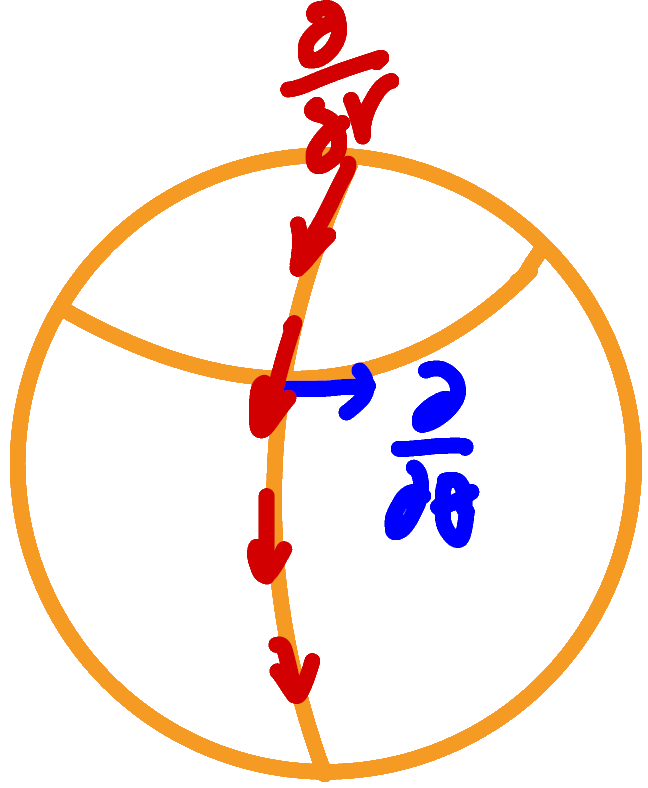
\includegraphics[scale=.2]{picture/week11/coordinate on S2.png}
    \end{center}
    Fixing \(\theta\), then \(\pdv{r}\) is the tangent vector field
    of the great circle, then 
    \[
        \frac{D}{dr}\left(\pdv{r}\right)=\nabla_{\pdv{r}}\pdv{r}
        =\Gamma\indices*{_{rr}^r}\pdv{r}+\Gamma\indices*{_{rr}^\theta}
        \pdv{\theta},
    \]
    where
    \[
        \Gamma\indices*{_{rr}^r}=\frac{1}{2}g^{rk}\left(
            \pdv{g_{rk}}{r}+\pdv{g_{rk}}{r}-\pdv{g_{rr}}{x^k}
        \right)
        =\frac{1}{2}g^{rr}\pdv{g_{rr}}{r}=0.
    \]
    \[
        \Gamma\indices*{_{rr}^\theta}=\frac{1}{2}
        g^{\theta\theta}\left(
            \pdv{g_{r\theta}}{r}
            +\pdv{g_{r\theta}}{r}
            -\pdv{g_{rr}}{\theta}
        \right)
        =0    
    \]
    \(\Rightarrow\frac{D}{dr}\pdv{r}=0\Rightarrow\) \(\pdv{r}\)
    is parallel along itself.

    If we compute 
    \[
        \frac{D}{d\theta}\pdv{\theta}=\nabla_{\pdv{\theta}}\pdv{\theta}
        =\Gamma\indices*{_{\theta\theta}^r}\pdv{r}+\Gamma
        \indices*{_{\theta\theta}^\theta}\pdv{\theta}
        =-\sin r\cos r \pdv{r}.    
    \]
    Hence, 
    \[
        \textcolor{blue}{
            \frac{D}{d\theta}\pdv{\theta}=0
            \Longleftrightarrow r=\frac{\pi}{2}.}
    \]
\end{remark}
\underline{Facts}:
\[
    \frac{DV(t)}{dt}=0\Longleftrightarrow 
    \dot{V}^i(t)+\Gamma\indices*{_{jk}^i}(t)\dot{x}^j(t)V^k(t)=0.    
\]
This is the \engordnumber{1} order linear O.D.E. system of
\(V(t)\). Hence, given a curve \(\alpha(t)\), let \(p\in\alpha(t)\),
\(v_0\in T_p M\), then by the Solution to the Cauchy problem, there is 
a unique parallel vector field \(V(t)\) along \(\alpha(t)\) such that 
\(V(0)=v_0\). 
\begin{center}
    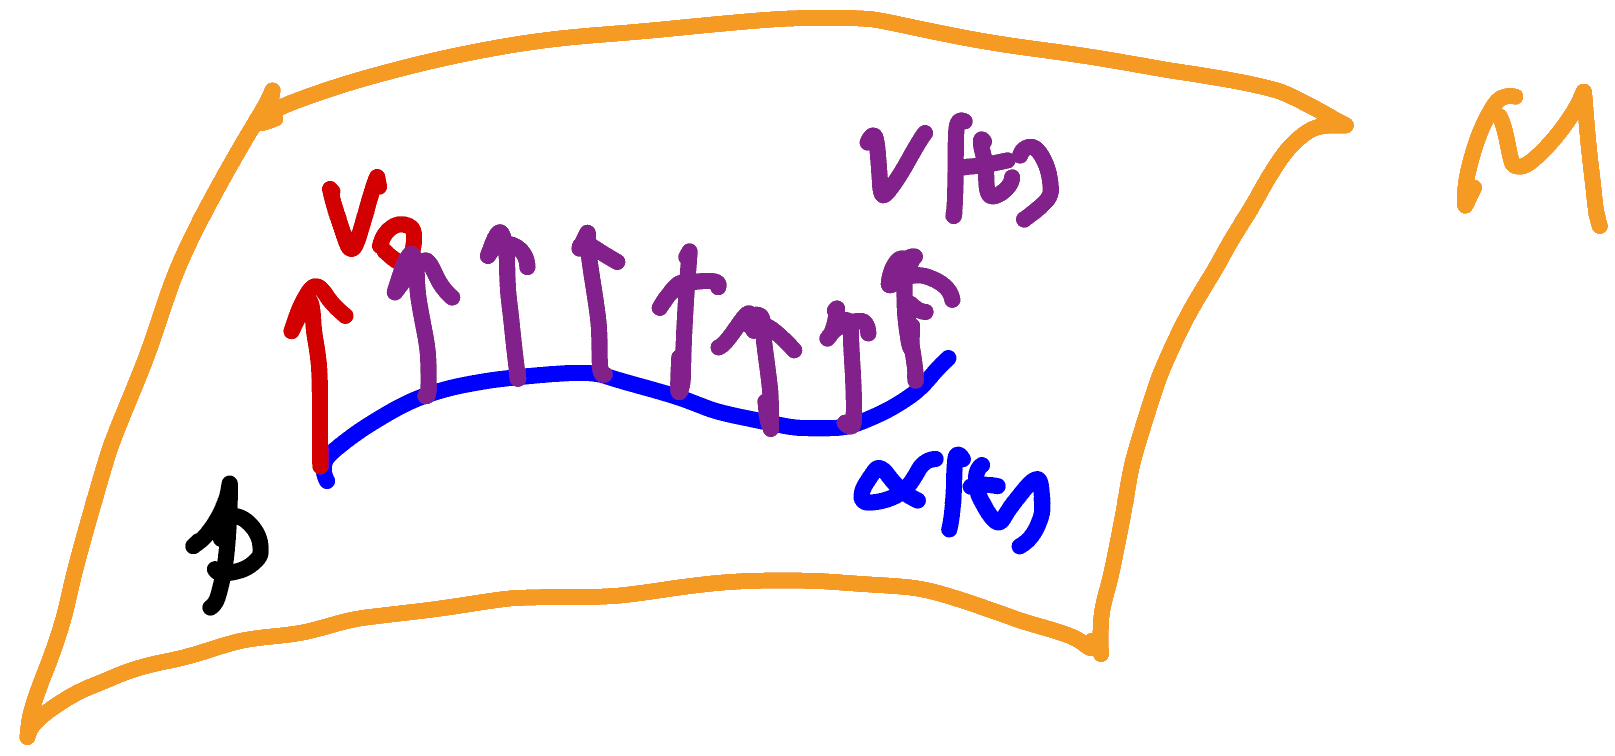
\includegraphics[scale=0.25]{picture/week11/parallel transport.png}
\end{center}
Consider \(p,q\in M\), let \(\alpha(t)\colon[0,1]\to M\) such that 
\(\alpha(0)=p,\alpha(1)=q,v_0\in T_p M\), and \(V(t)\) is the parallel 
vector field along \(\alpha(t)\) with \(V(0)=v_0\), then 
\textcolor{blue}{
    \(V(1)\in T_q M\) is called the parallel transportation of 
    \(v_0\) at \(q\).
}
\textcolor{blue}{
    \begin{proposition}
        Let \(V_1,V_2\) be two parallel vector fields along a curve 
        \(\alpha(t)\), then \(\left\langle V_1,V_2 \right\rangle\)
        is a constant along \(\alpha(t)\).
    \end{proposition}
}
\begin{proof}
    \(\dv{t}\left\langle V_1(t),V_2(t)\right\rangle
    =\left\langle\dv{V_1(t)}{t},V_2(t)\right\rangle
    +\left\langle\dv{V_2(t)}{t},V_1(t)\right\rangle
    =0\).
\end{proof}
\textcolor{blue}{
    \begin{corollary}
        The parallel transport along a curve does not
        change the length or angle of original vectors.
        \begin{center}
            \includegraphics[scale=0.2]{picture/week11/p. transport 
            isometry.png}
        \end{center}
        In particular, the map 
        \[  
            P_{\alpha(1)}\colon T_p M\to T_q M
        \]
        is a linear isometry.
    \end{corollary}
}
\begin{remark}
    The advantage of parallel transport is helping us choose an
    orthonormal frame along a curve \(\alpha(t)\). At \(T_p M\),
    choose orthonormal basis \{\(E_1,\ldots,E_n\)\} and parallel
    transport \(E_i\) along \(\alpha\), then at each point 
    of the curve \(\{E_1(t),\ldots,E_n(t)\}\)is an orthonormal basis
    of \(T_{\alpha(t)}M\).
    \begin{center}
        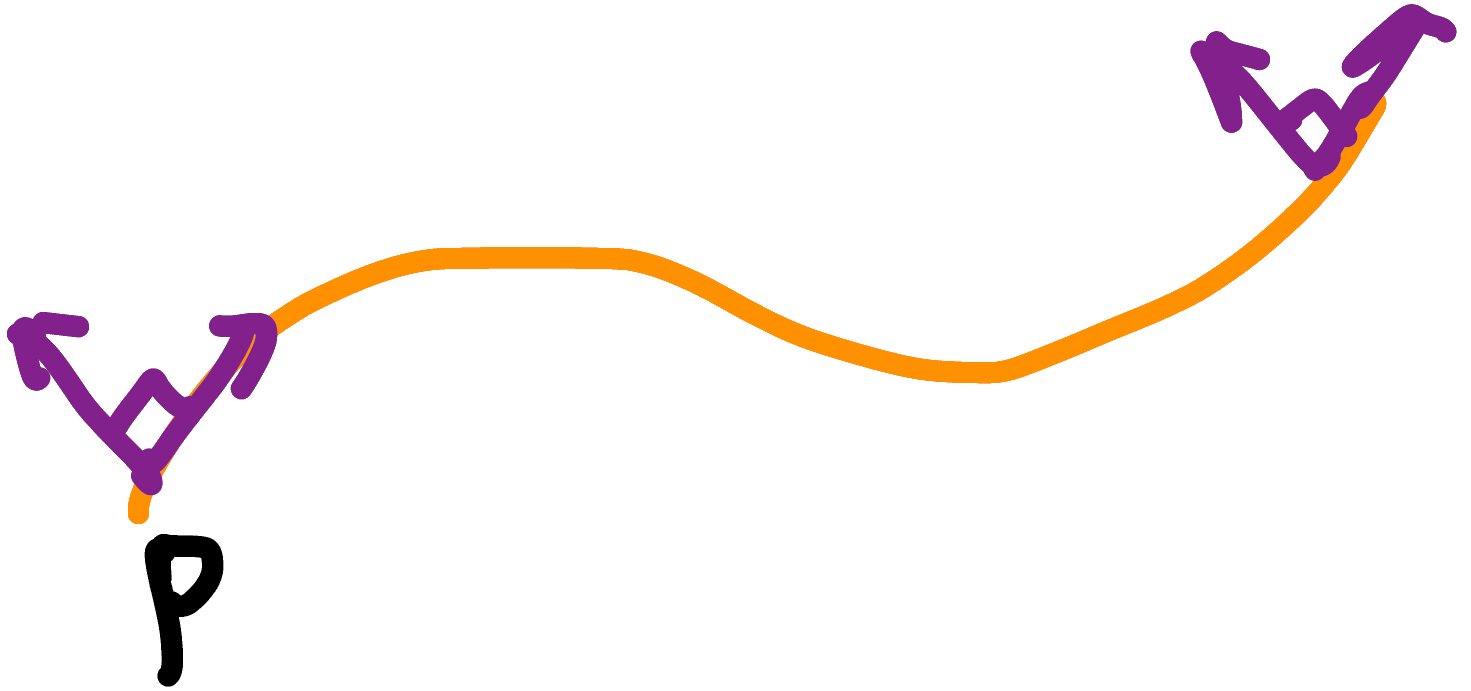
\includegraphics[scale=0.15]{picture/week11/orthonormal basis.png}
    \end{center}
    For any vector field \(V(t)\) along
    \(\alpha(t)\), \textcolor{blue}{\(V(t)=V^i(t)E_i(t)\)},
    \[
        \frac{DV(t)}{dt}=\frac{D}{dt}\left(
            V^i(t)E_i(t)
        \right)    
        =\dot{V}^i(t)E_i(t)+V^i(t)\underbrace{\frac{DE_i(t)}{dt}}_{=0}.
    \]
    \[
        \frac{DV(t)}{dt}=\dot{V}^i(t)E_i(t).
    \]
\end{remark}
\begin{remark}
    \(\forall p\in M\), let \(\alpha\) be a piecewise 
    smooth \textcolor{blue}{closed} curve  passing through \(p\),
    then the parallel transport \(P_\alpha\colon T_p M\to T_p M\)
    yields a linear isometry of \(T_p M\). If \(\beta\) is another
    piecewise \textcolor{blue}{closed} curve passing through \(p\),
    we have another linear isometry \(P_\beta\).
\end{remark}
\textcolor{blue}{
    \begin{definition}
        \[\mathrm{Hol}_p(M,g)=\{P_\alpha\colon T_p M\to T_p M,
        \alpha\text{: closed curve passing
        through }p\}.\]
        \begin{center}
            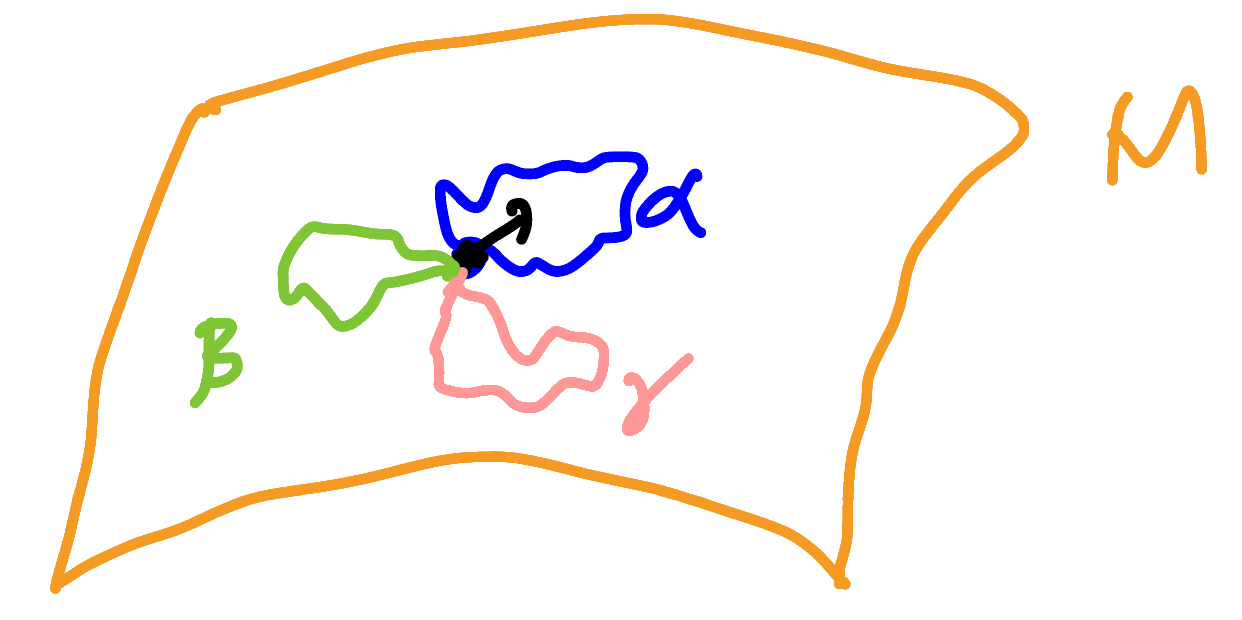
\includegraphics[scale=0.3]{picture/week11/holonomy groups.png}
        \end{center}
    \end{definition}
}
This set has a group structure given by composition of parallel transport.
\(\mathrm{Hol}_p(M,g)\) is called the Holonomy group of \(M\) at \(p\).
In fact, it's a Lie group. Note that \(\mathrm{Hol}(M,g)\) relies on 
the Riemannian metric \(g\).\

\textcolor{cyan}{
    {\Large \textbf{!}} The classification of Holonomy group is useful 
    to understand the classification of Riemannian manifold (metric). 
    Details can be found in Peter Perterson's Riemannian Geometry
    book p.388.
}
\textcolor{blue}{
    \begin{definition}[Geodesics]
        \(\gamma(t)\) is a parametrized curve in \(M\), if
        \[
            \frac{D}{dt}\dot{\gamma}(t)=0\left(\Longleftrightarrow
            \nabla_{\dot{\gamma}(t)}\dot{\gamma}(t)=0
            \text{ or simply }\nabla_{\dot{\gamma}}\dot{\gamma}\right).    
        \]
        \ie\ \(\dot{\gamma}(t)\) is a parallel vector field along
        \(\gamma(t)\), then we call \(\alpha(t)\) a geodesic. 
    \end{definition}
}
\begin{remark}
    By definition, \(\left\langle\dot{\gamma}(t),\dot{\gamma}(t)
    \right\rangle\) is constant, after reparametrization,
    \(\gamma(t)=\gamma(s),s=ct\) is the arclength parameter,
    \(\therefore\) a curve \(\alpha(s)\) with arclength parameter
    is a geodesic iff \(\frac{D}{ds}\left(\alpha'(s)\right)=0\).
\end{remark}
\subsection{Geodesics on surfaces}
Let \(S\) be a regular surface in \(\mathbb{R}^3\). Let \(\alpha(s)\)
be a geodesic on \(S\) with arclength parameter. Then \(\alpha''(s)\)
(in \(\mathbb{R}^3\)) has the following decomposition
\begin{align*}
    \alpha''(s)&=\frac{D}{ds}\left(\alpha'(s)\right)+
    \left\langle\alpha''(s),\va*{N}\left(\alpha(s)\right)\right\rangle
    \va*{N}\\
    &=\left\langle\alpha''(s),\va*{N}\left(\alpha(s)\right)\right\rangle
    \va*{N}\\
    &=k_{\vb{n}}(s)\va*{N}.\footnotemark
\end{align*}
\footnotetext{Recall that \(k_{\vb{n}}(s)=\II \left(\alpha'(s),
\alpha'(s)\right)\).}
\(\therefore \alpha(s)\) is a geodesic \(\Longleftrightarrow\) principal
normal \(\va{n}(s)\) is parallel to the normal of surface \(\va*{N}\).
Note normal section is a geodesic, but geodesic may not be a normal
section.
\begin{enumerate}[(1)]
    \item \(\mathbb{S}^2\). Great circles are geodesics.
    \begin{center}
            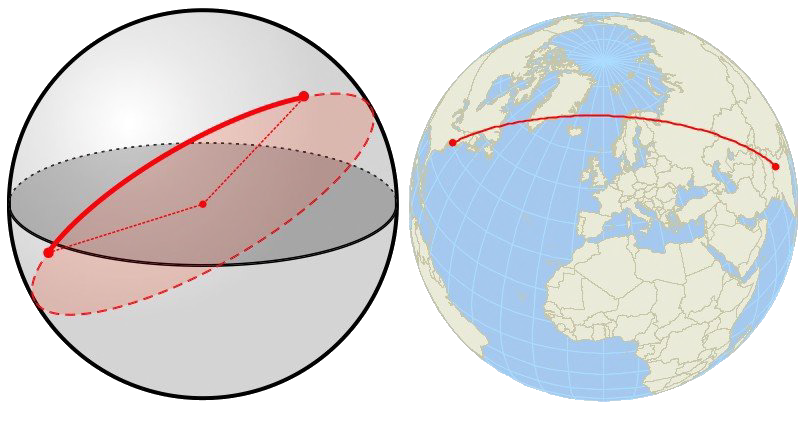
\includegraphics[scale=0.7]{picture/week11/geodesics on S2.png}
    \end{center}
    \item On Cylinder, \(x^2+y^2=1\), 
    \begin{center}
        \includegraphics[scale=0.5]{picture/week11/geodesics on 
        cylinder.png}
    \end{center}
    consider the local parametrization
    \[\gamma(u,v)=\left(\cos u ,\sin u,v\right)\]
    \(\Rightarrow\) lines, horizontal circles, and helix curve
    \(\left(\cos as,\sin as, bs\right)\) are all geodesics.
\end{enumerate}
